\documentclass[aspectratio=169,10pt]{ctexbeamer}

\usetheme{Madrid}
\usecolortheme{default}
\usefonttheme{professionalfonts}

\usepackage{amsmath,amssymb}
\usepackage{booktabs}
\usepackage{graphicx}
\usepackage{tikz}
\usepackage{array}
\usepackage{xcolor}

\definecolor{zjublue}{RGB}{0,63,136}
\definecolor{zjuorange}{RGB}{214,118,0}
\definecolor{softgreen}{RGB}{0,128,96}
\setbeamercolor{palette primary}{bg=zjublue,fg=white}
\setbeamercolor{palette secondary}{bg=zjublue!85,fg=white}
\setbeamercolor{palette tertiary}{bg=zjublue!70,fg=white}
\setbeamercolor{structure}{fg=zjublue}
\setbeamercolor{frametitle}{bg=zjublue,fg=white}
\setbeamertemplate{navigation symbols}{}
\setbeamertemplate{caption}[numbered]

\title[CTQW Quantum-Guided Greedy]{连续时间量子游走辅助贪心算法}
\subtitle{面向最大团问题的量子启发式图优化实验}
\author{浙江大学量子信息课程项目组}
\institute{ZJU Quantum Information}
\date{2025年6月15日}

\newcommand{\ctqw}{\mathrm{CTQW}}
\newcommand{\score}{\mathrm{Score}}
\newcommand{\qscore}{Q_{\mathrm{norm}}}
\newcommand{\rscore}{R_{\mathrm{norm}}}

\begin{document}

\begin{frame}
  \titlepage
\end{frame}

\begin{frame}{汇报主线}
  \tableofcontents
\end{frame}

\section{研究问题}

\begin{frame}{问题背景：最大团问题}
  \begin{columns}[T,onlytextwidth]
    \begin{column}{0.60\textwidth}
      \begin{block}{Maximum Clique Problem}
        给定无向图 $G=(V,E)$，寻找尽可能大的节点集合 $S\subseteq V$，满足
        \[
          \forall u,v\in S,\ u\neq v,\ (u,v)\in E.
        \]
      \end{block}
      \vspace{0.4em}
      \begin{itemize}
        \item 经典 NP-hard 组合优化问题
        \item 近似方法：从一个起点出发，逐轮加入合法候选节点
        \item 关键瓶颈：每一轮如何在候选集合中选择下一个节点
      \end{itemize}
    \end{column}
    \begin{column}{0.40\textwidth}
      \centering
      \vspace{0.3em}
      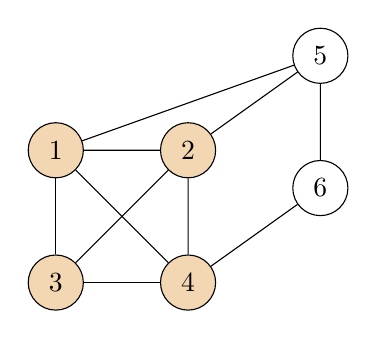
\begin{tikzpicture}[scale=1.20, every node/.style={circle, draw, minimum size=7mm}]
        \node[fill=zjuorange!30] (a) at (0,1.4) {1};
        \node[fill=zjuorange!30] (b) at (1.4,1.4) {2};
        \node[fill=zjuorange!30] (c) at (0,0) {3};
        \node[fill=zjuorange!30] (d) at (1.4,0) {4};
        \node (e) at (2.8,2.4) {5};
        \node (f) at (2.8,1.0) {6};
        \foreach \x/\y in {a/b,a/c,a/d,b/c,b/d,c/d,a/e,b/e,d/f,e/f}
          \draw (\x) -- (\y);
      \end{tikzpicture}
      \vspace{0.7em}

      \small 橙色节点构成 4 阶团
    \end{column}
  \end{columns}
\end{frame}

\begin{frame}{核心研究问题}
  \begin{block}{传统贪心的局限}
    度数和候选子图度数主要反映局部邻域结构，难以表达多跳路径、整体连通性和全局拓扑。
  \end{block}

  \vspace{0.8em}
  \begin{alertblock}{本项目问题}
    连续时间量子游走（CTQW）产生的节点概率分布，能否作为一种全局结构信号，
    辅助贪心算法找到更高质量的团？
  \end{alertblock}

  \vspace{0.8em}
  \begin{itemize}
    \item 若 CTQW 能突出团区域，则可作为节点评分信号
    \item 若量子信号与经典评分互补，则混合贪心可能更稳健
    \item 若嵌入式方案失败，需要诊断失败来自量子模型本身还是使用方式
  \end{itemize}
\end{frame}

\section{基本原理}

\begin{frame}{连续时间量子游走}
  \begin{block}{量子态在图上的表示}
    将图节点与 Hilbert 空间基矢量一一对应：
    $|1\rangle,|2\rangle,\ldots,|n\rangle$，
    系统状态为这些基的复系数叠加：
    \[
      |\psi(t)\rangle = \sum_{v\in V} \alpha_v(t)\,|v\rangle,
      \qquad
      P_v(t) = |\alpha_v(t)|^2 = |\langle v|\psi(t)\rangle|^2
    \]
  \end{block}

  \vspace{0.1em}

  \begin{block}{演化方程与形式解}
    CTQW 遵循薛定谔方程（取 $\hbar=1$）：
    \[
      i\frac{\partial}{\partial t}|\psi(t)\rangle = H|\psi(t)\rangle
      \quad\Longrightarrow\quad
      |\psi(t)\rangle = e^{-iHt}\,|\psi_0\rangle
    \]
    $U(t)=e^{-iHt}$ 为时间演化算子（幺正矩阵）。$H$ 由图邻接矩阵 $A$
    及种子扰动项 $\lambda\sum_{u\in S}|u\rangle\langle u|$ 构造，是 Hermitian 矩阵$^{*}$。
  \end{block}

  {\small $^{*}\;H$ 的 Hermitian 性质保证了 $U^\dagger U=I$，从而
  $\sum_v P_v(t)=1$——CTQW 输出的概率分布天然合法，可直接用作节点评分信号。}
\end{frame}

\begin{frame}{CTQW 全局感知}
  \begin{columns}[T,onlytextwidth]
    \begin{column}{0.60\textwidth}
      \begin{block}{泰勒展开}
        \[
          e^{-iHt} = I + (-it)H + \frac{(-it)^2}{2!}H^2
                   + \frac{(-it)^3}{3!}H^3 + \cdots
        \]
        取 $H=A$（图邻接矩阵），则 $(A^k)_{uv}=u$ 到 $v$ 的长度为 $k$ 路径条数
      \end{block}
    \end{column}

    \begin{column}{0.37\textwidth}
      \centering
      \vspace{0.4em}
      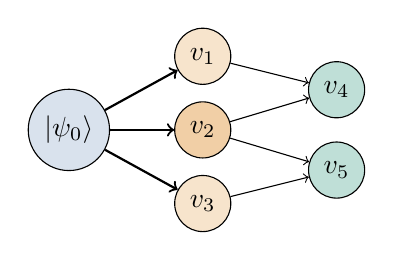
\begin{tikzpicture}[scale=0.85]
        \node[circle,draw,fill=zjublue!15] (s) at (0,0) {$|\psi_0\rangle$};
        \node[circle,draw,fill=zjuorange!20] (a) at (2,1.1) {$v_1$};
        \node[circle,draw,fill=zjuorange!35] (b) at (2,0) {$v_2$};
        \node[circle,draw,fill=zjuorange!20] (c) at (2,-1.1) {$v_3$};
        \node[circle,draw,fill=softgreen!25] (d) at (4,0.6) {$v_4$};
        \node[circle,draw,fill=softgreen!25] (e) at (4,-0.6) {$v_5$};
        \draw[->,thick] (s) -- (a);
        \draw[->,thick] (s) -- (b);
        \draw[->,thick] (s) -- (c);
        \draw[->] (a) -- (d);
        \draw[->] (b) -- (d);
        \draw[->] (b) -- (e);
        \draw[->] (c) -- (e);
      \end{tikzpicture}
      \vspace{0.5em}

      \small 多条路径的概率幅在目标区域相干叠加
    \end{column}
  \end{columns}

  \vspace{1.5em}

  \small
  \renewcommand{\arraystretch}{1.4}
  \setlength{\tabcolsep}{4pt}
  \begin{tabular}{p{0.15\textwidth}p{0.26\textwidth}p{0.26\textwidth}p{0.26\textwidth}}
    \toprule
    & 度数评分 & 经典随机游走 & CTQW \\
    \midrule
    信息来源 & 只看 $k{=}1$ 邻居 & 各阶路径概率加权和 & 各阶路径\alert{复振幅}相干叠加 \\
    干涉效应 & 无 & 无 & 有（相干增强或抵消）\\
    \bottomrule
  \end{tabular}
\end{frame}

\section{算法设计}

\begin{frame}{实验二算法总览}
  \begin{alertblock}{ClassicalClique —— 候选子图度数贪心（强基线）}
    $\operatorname{Score}(v,S)=\deg_{C(S)}(v)$，每轮随 $S$ 变化重新计算候选节点在
    候选诱导子图中的度数。衡量的是"选 $v$ 后还剩多少可扩展的合法候选"，是本项目所有实验的统一参照对象。
  \end{alertblock}

  \vspace{0.15em}

  \begin{block}{ClassicalDegree —— 全图度数贪心（弱基线）}
    $\operatorname{Score}(v)=\deg(v)$，仅计算一次，所有轮迭代复用同一套分数。
    不感知候选集合约束，不随部分解 $S$ 动态调整。
  \end{block}

  \vspace{0.15em}

  \begin{block}{SimulatedAnnealing —— 模拟退火（经典概率基线）}
    以概率 $e^{-\Delta/T}$ 接受劣解，温度 $T$ 逐步下降。
    经典非贪心启发式方法，可跳出局部最优，代表纯经典方案在非贪心框架下的上限。
  \end{block}
\end{frame}

\begin{frame}{量子引导贪心}
  \begin{block}{最大团候选集合}
    \[
      C(S)=\{v\in V\setminus S\mid \forall u\in S,\ (u,v)\in E\}.
    \]
    先限制合法候选节点，保证输出始终为团。
  \end{block}

  \vspace{0.6em}
  \begin{block}{混合评分函数}
    \[
      \score(v,S)=\alpha \qscore(v,S)+(1-\alpha)\rscore(v,S).
    \]
  \end{block}

  \begin{itemize}
    \item $\qscore$：CTQW 概率的归一化结果，提供全局结构信号
    \item $\rscore$：候选诱导子图度数的归一化结果，提供局部可扩展性
    \item $\alpha=0$ 为纯经典，$\alpha=1$ 为纯量子
  \end{itemize}
\end{frame}

\begin{frame}{实验三算法总览}
  三个 MultiStart 变体共用同一骨架：$K$ 个起点各自独立运行 ClassicalCliqueGreedy，
  取最优结果。唯一差异在于起点集合的选取方式。

  \vspace{0.25em}

  \begin{block}{MultiStartRandom($K$)：随机起点}
    从 $V$ 中均匀随机抽取 $K$ 个节点作为起点集合。
    若目标算法不显著优于此基线，则"多起点"本身即足以解释性能提升。
  \end{block}

  \vspace{0.15em}

  \begin{block}{MultiStartDegree($K$)：度数 Top-$K$ 起点}
    取全图度数最高的 $K$ 个节点作为起点集合。
    若目标算法不显著优于此基线，则 CTQW 未提供度数之外的额外信息。
  \end{block}

  \vspace{0.15em}

  \begin{alertblock}{MultiStartCTQW($K$)：CTQW 概率 Top-$K$ 起点}
    一次全图均匀叠加 CTQW 演化（$|\psi_0\rangle{=}\frac{1}{\sqrt{n}}\sum_v|v\rangle$，$H{=}A$），
    取概率最高的 $K$ 个节点作为起点集合。
    待验证：CTQW 能否提供独立于度数的全局结构信号。
  \end{alertblock}
\end{frame}

\section{实验结果}

\begin{frame}{三组实验设计}
  \centering
  \renewcommand{\arraystretch}{1.25}
  \begin{tabular}{p{0.20\textwidth}p{0.46\textwidth}p{0.22\textwidth}}
    \toprule
    实验 & 验证问题 & 结论 \\
    \midrule
    实验一 & CTQW 能否识别图中的团结构 & 成立 \\
    实验二 & 将 CTQW 嵌入每轮贪心，混合评分是否更稳健 & 部分成立 \\
    实验三 & 将 CTQW 外置为起点选择器，能否超越强经典基线 & 成立 \\
    \bottomrule
  \end{tabular}

  \vspace{1.5em}
  \begin{block}{总体结论}
    CTQW 的全局识别能力真实存在，但有效性强烈依赖使用方式：
    外置于贪心之前更有效，嵌入每轮局部扩散反而会污染经典评分。
  \end{block}
\end{frame}

\begin{frame}{工程实现工作量}
  \begin{columns}[T,onlytextwidth]
    \begin{column}{0.48\textwidth}
      \begin{block}{核心代码}
        \begin{itemize}
          \item \texttt{src/}：15 个 Python 模块
          \item \texttt{experiments/}：8 个实验脚本
          \item 核心算法与实验代码约 4450 行
          \item 实现 Classical / SA / Quantum / Multi-Start 四类求解器
        \end{itemize}
      \end{block}
    \end{column}
    \begin{column}{0.48\textwidth}
      \begin{block}{关键内容}
        \begin{itemize}
          \item 完成数据集收集和规范化，并配置相关可视化脚本
          \item 实现经典算法并搭建实验框架
          \item 完成真实 CTQW 矩阵指数演化
          \item 为经典贪心支持外部起点注入，完成 MultiStartCTQWGreedy 算法
        \end{itemize}
      \end{block}
    \end{column}
  \end{columns}

  \vspace{0.3em}

  \begin{columns}[T,onlytextwidth]
    \begin{column}{0.48\textwidth}
      \begin{block}{数据集与实验资产}
        \begin{itemize}
          \item 人工 planted 数据：220 个 JSON 实例
          \item 外部 DIMACS 转换数据：10 个 JSON 实例
          \item 配套数据生成、格式转换、可视化脚本
        \end{itemize}
      \end{block}
    \end{column}
    \begin{column}{0.48\textwidth}
      \begin{alertblock}{工作重点}
        不是只跑单个样例，而是建立了可复现实验框架：
        数据生成、算法实现、参数扫描、统计检验和图表输出均可复用
      \end{alertblock}
    \end{column}
  \end{columns}
\end{frame}

\begin{frame}{实验运行工作量}
  \centering
  \renewcommand{\arraystretch}{1.18}
  \begin{tabular}{p{0.32\textwidth}p{0.18\textwidth}p{0.14\textwidth}p{0.24\textwidth}}
    \toprule
    实验模块 & 任务/规模 & 运行次数 & 目的 \\
    \midrule
    CTQW 可视化 & MC, $n=30$ & 1 & 验证概率集中 \\
    嵌入式算法对比 & MC small & 1040 & 对比强经典基线 \\
    $\alpha$ 参数扫描 & MC small/medium & 4540 & 定位权重敏感性 \\
    组件消融 & MC small & 1040 & 拆分 Q/R/$\lambda$ 贡献 \\
    DS 补充实验 & DS small & 2880 & 验证另一类图任务 \\
    Multi-Start 起点选择 & MC small/medium & 5840 & 验证外置 CTQW 方案 \\
    \bottomrule
  \end{tabular}

  \vspace{1em}
  \begin{alertblock}{总量}
    累计约 18,300 次算法运行；显著性检验采用 Wilcoxon signed-rank paired test，
    按 \texttt{sample\_id, run\_id} 严格配对。
  \end{alertblock}
\end{frame}

\begin{frame}{实验一：CTQW 能突出 planted clique}
  \small 数据：$n=30,p=0.1,k=5$ 植入团，
  指标：$\displaystyle Ratio=\frac{\mathrm{Mean}(P_v,\ v\in S_*)}{\mathrm{Mean}(P_v,\ v\notin S_*)}$.

  \vspace{0.3em}

  \centering
  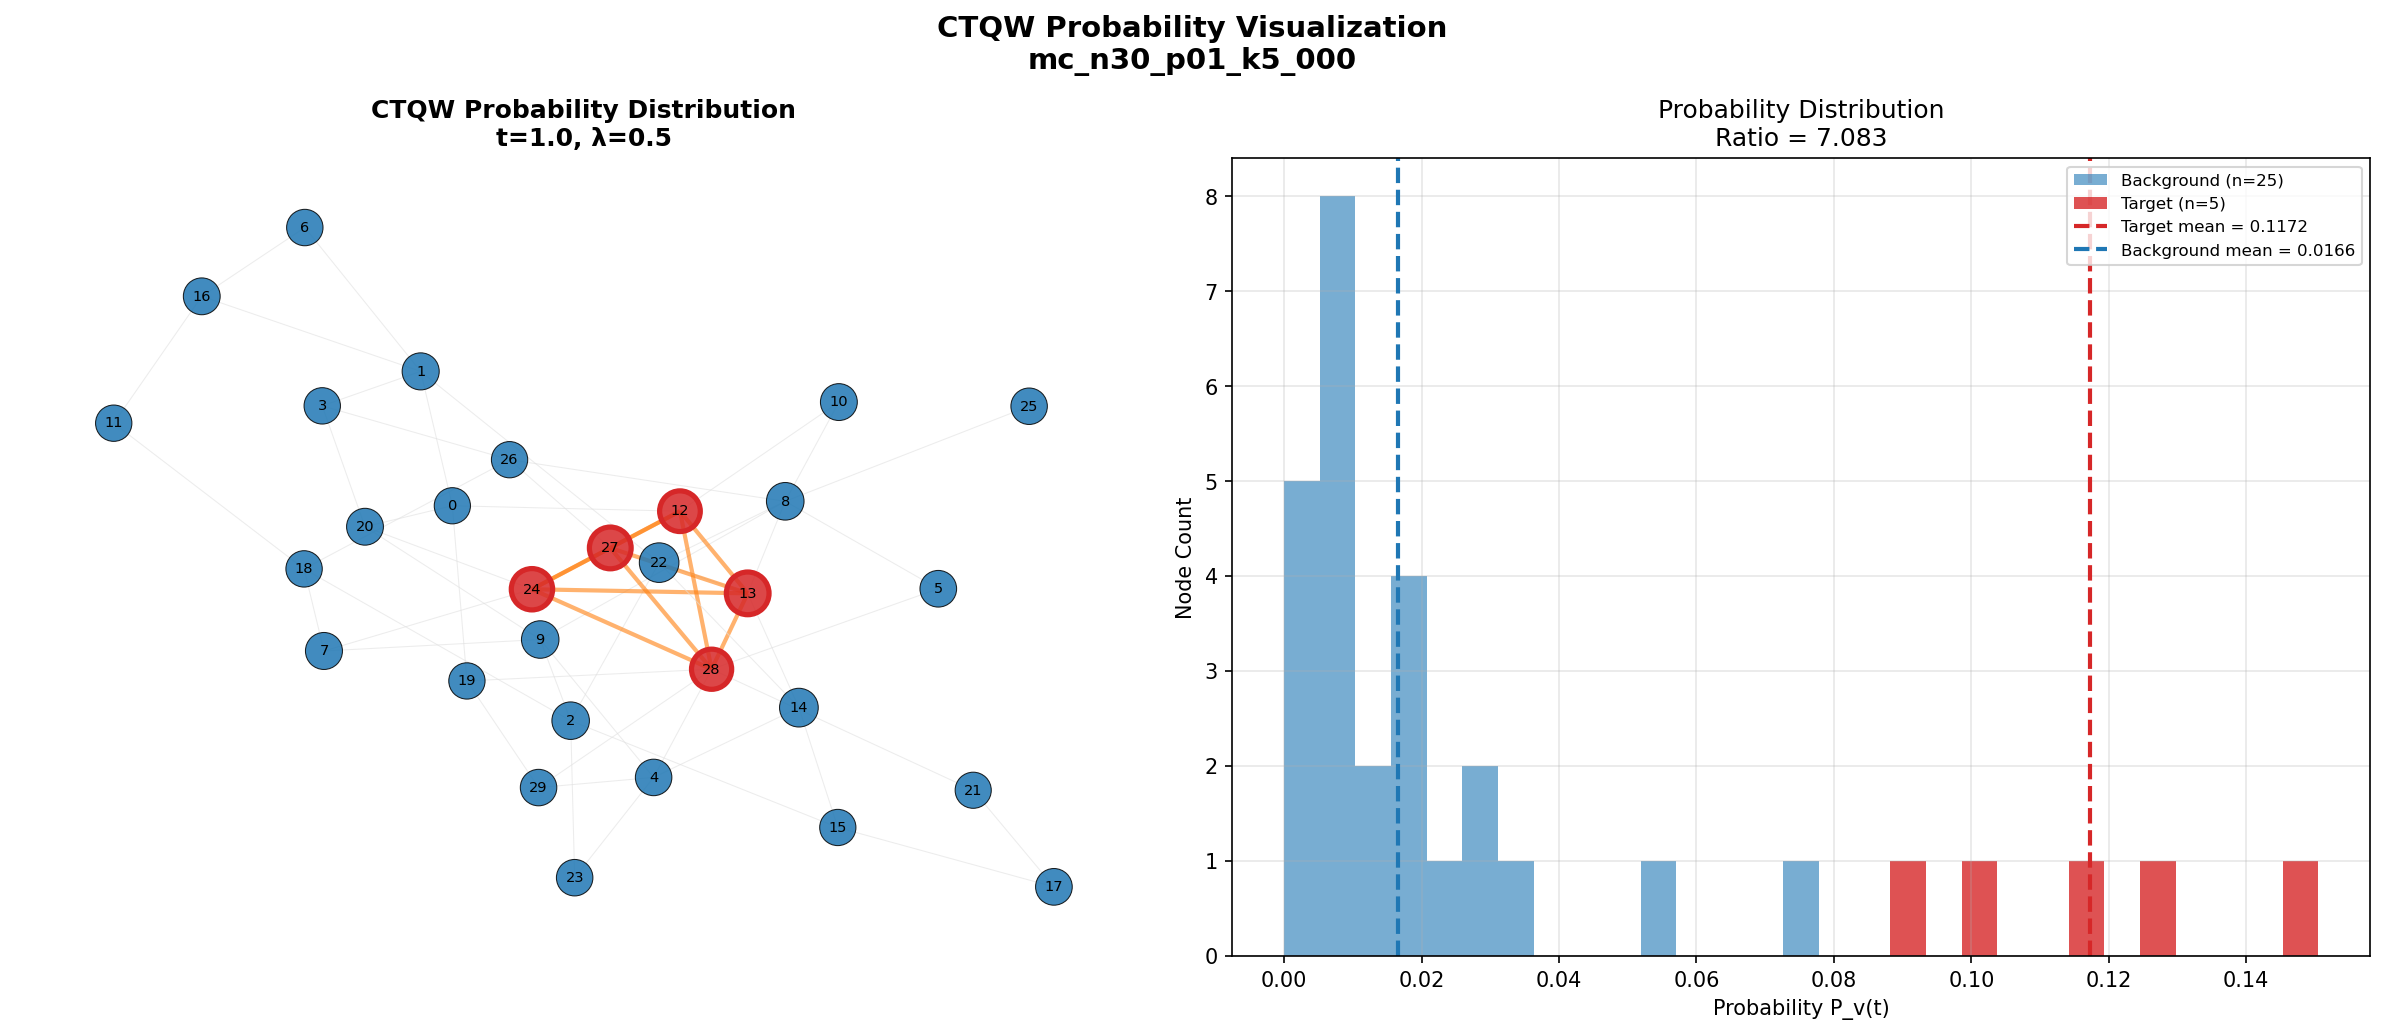
\includegraphics[height=4.6cm,width=0.80\linewidth]{images/visual_probability.png}

  \vspace{0.3em}

  \begin{alertblock}{实验结果}
    团节点平均概率 $0.1172$，背景节点平均概率 $0.0166$，Ratio $=7.08$。
    CTQW 在植入团区域形成显著概率集中，团节点平均概率约为背景节点的 7 倍。
  \end{alertblock}
\end{frame}

\begin{frame}{实验一补充：CTQW 不只是复述度数}
  \centering
  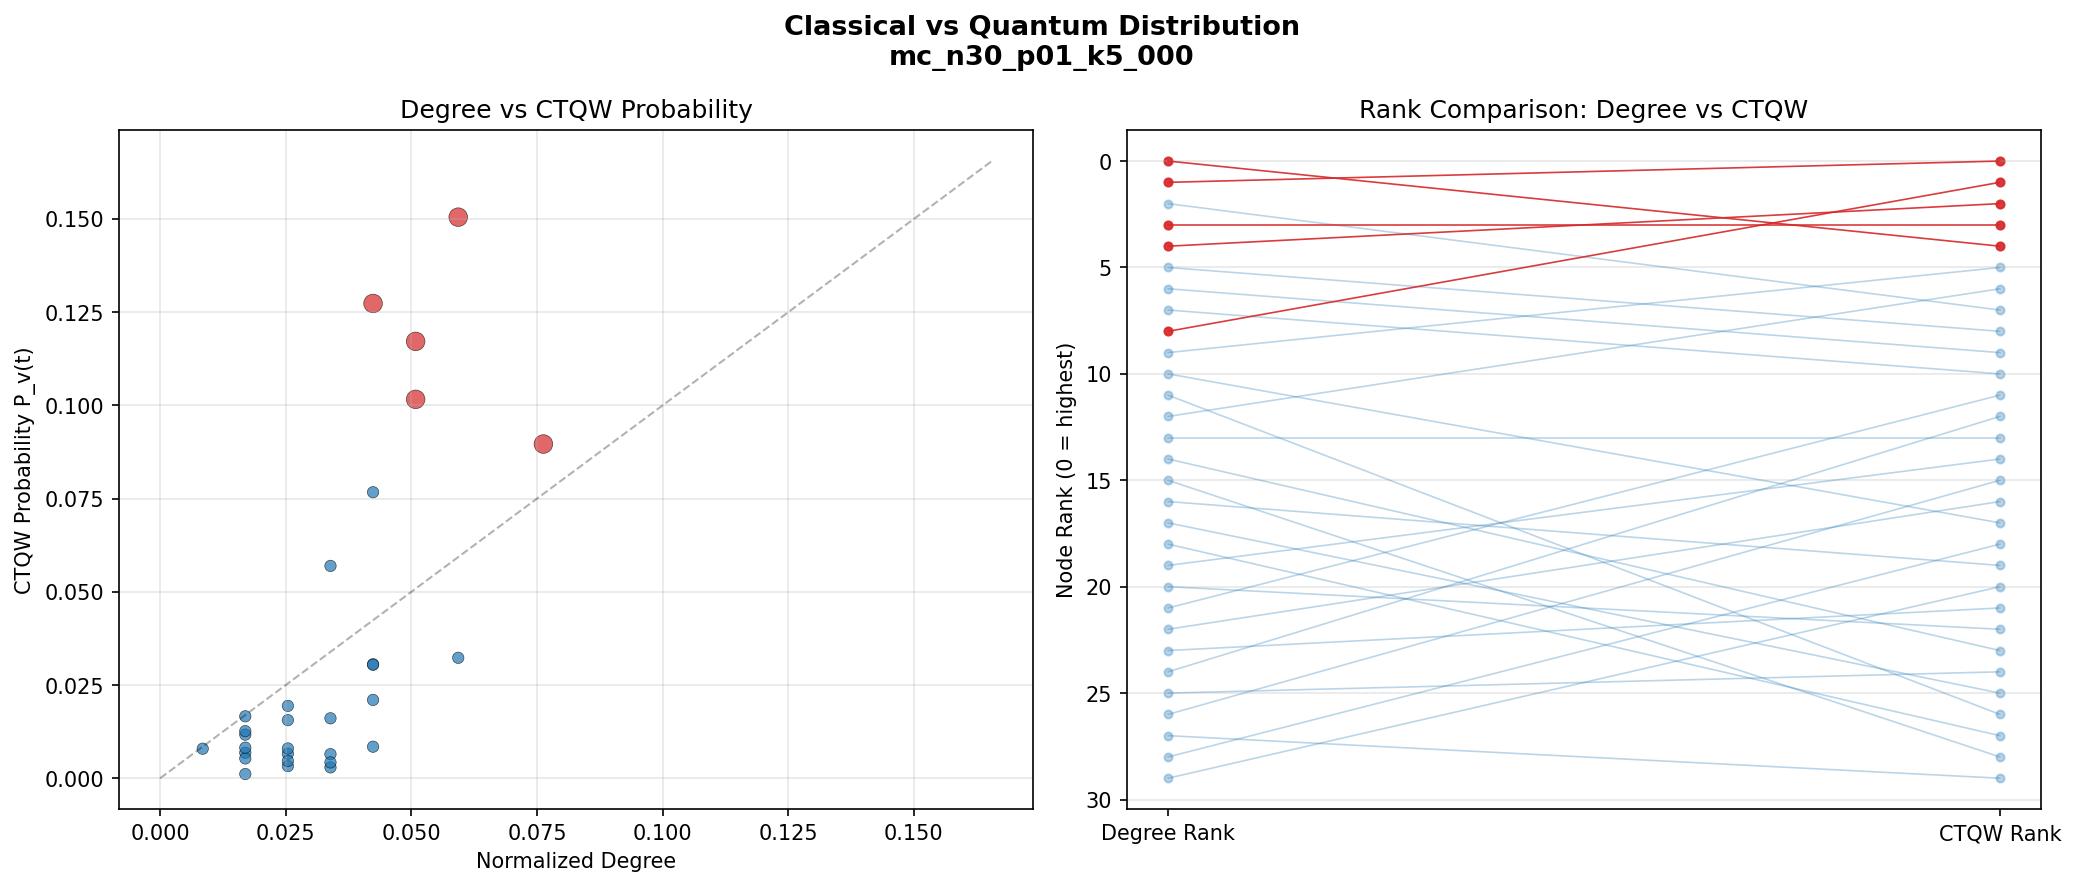
\includegraphics[width=0.85\linewidth]{images/Classical_vs_Quantum.png}

  \vspace{0.4em}

  \begin{itemize}
    \item 横轴为归一化度数，纵轴为归一化 CTQW 概率
    \item 5 个团节点全部位于对角线上方，说明 CTQW 对团结构给出超出度数的概率放大
    \item \textbf{CTQW 具备识别图全局团结构的能力，基础假设成立。}
  \end{itemize}
\end{frame}

\begin{frame}{实验二：嵌入式 CTQW 未超越经典强基线}
  \begin{columns}[T,onlytextwidth]
    \begin{column}{0.49\textwidth}
      \centering
      \begin{tabular}{lcc}
        \toprule
        算法 & 团大小 & $\Delta$ \\
        \midrule
        ClassicalClique & \textbf{7.20} & -- \\
        QuantumGuidedGreedy & 6.71 & -0.49 \\
        ClassicalDegree & 6.66 & -0.54 \\
        SimulatedAnnealing & 6.50 & -0.70 \\
        \bottomrule
      \end{tabular}
      \vspace{0.4em}

      \small small 规模，均值结果
    \end{column}
    \begin{column}{0.47\textwidth}
      \centering
      \begin{tabular}{lcc}
        \toprule
        $\alpha$ & 团大小 & $\Delta$ \\
        \midrule
        0.00 & 7.20 & 0.00 \\
        0.25 & 7.14 & -0.06 \\
        0.50 & 6.71 & -0.49 \\
        0.75 & 5.08 & -2.12 \\
        1.00 & 4.65 & -2.55 \\
        \bottomrule
      \end{tabular}
      \vspace{0.4em}

      \small $\alpha$ 越高，性能越差
    \end{column}
  \end{columns}

  \vspace{1em}
  \begin{alertblock}{结论}
    混合方案显著优于纯量子，但仍落后于纯经典；嵌入式方案只“部分成立”。
  \end{alertblock}
\end{frame}

\begin{frame}{实验二分析：局部扩散覆盖全局优势}
  \begin{columns}[T,onlytextwidth]
    \begin{column}{0.47\textwidth}
      \begin{block}{实验一的初始态}
        \[
          |\psi_0\rangle=\frac{1}{\sqrt{|V|}}\sum_{v\in V}|v\rangle
        \]
        全图均匀叠加，回答“图中哪里结构最显著”。
      \end{block}
    \end{column}
    \begin{column}{0.47\textwidth}
      \begin{block}{嵌入式贪心的初始态}
        \[
          |\psi_0\rangle=\frac{1}{\sqrt{|S|}}\sum_{u\in S}|u\rangle
        \]
        从已选集合出发，回答“哪些节点离当前种子更近”。
      \end{block}
    \end{column}
  \end{columns}

  \vspace{1em}
  \begin{itemize}
    \item 嵌入式 CTQW 做的是局部种子扩散
    \item 经典候选子图度数也在衡量局部可扩展性
    \item $Q$ 与 $R$ 回答的问题相近，但 $Q$ 受相位干涉影响更不稳定
  \end{itemize}
\end{frame}

\begin{frame}{实验三：CTQW 作为外部起点选择器}
  \begin{block}{MultiStartCTQWGreedy}
    \begin{enumerate}
      \item 用全图均匀初态运行一次 CTQW
      \item 选取概率最高的 $K$ 个节点作为候选起点
      \item 从每个起点独立运行 ClassicalCliqueGreedy
      \item 返回最优结果
    \end{enumerate}
  \end{block}

  \vspace{0.6em}

  \begin{itemize}
    \item 保留实验一已验证有效的全局初始态
    \item 避免每轮局部扩散污染经典评分
    \item 使用 Random Top-K 与 Degree Top-K 进行对照
  \end{itemize}
\end{frame}

\begin{frame}{实验三结果：显著超越强经典基线}
  \centering
  \renewcommand{\arraystretch}{1.25}
  \begin{tabular}{lccc}
    \toprule
    算法 & 团大小 $\mu\pm\sigma$ & $\Delta$ vs 基线 & $p$-value \\
    \midrule
    ClassicalClique & $11.70\pm4.31$ & -- & -- \\
    MultiStartRandom(K=10) & $9.91\pm4.64$ & -1.80 & $<0.001$ \\
    MultiStartDegree(K=10) & $12.38\pm3.55$ & +0.68 & $<0.001$ \\
    \textbf{MultiStartCTQW(K=10)} & $\mathbf{12.41\pm3.52}$ & \textbf{+0.71} & $\mathbf{<0.001}$ \\
    \bottomrule
  \end{tabular}

  \vspace{1.2em}
  \begin{block}{结论}
    将 CTQW 放在贪心外部作为起点选择器，在 small 与 medium 两个规模上均
    显著超越 ClassicalClique 强基线。
  \end{block}
\end{frame}

\begin{frame}{结果边界：CTQW 与度数信号高度相关}
  \begin{columns}[T,onlytextwidth]
    \begin{column}{0.50\textwidth}
      \begin{tabular}{lccc}
        \toprule
        规模 & K & CTQW-Degree & $p$ \\
        \midrule
        small & 1 & -0.52 & $<0.001$ \\
        small & 3 & +0.05 & 0.010 \\
        small & 5 & +0.02 & 0.046 \\
        small & 10 & 0.00 & 1.000 \\
        medium & 10 & +0.03 & 0.046 \\
        \bottomrule
      \end{tabular}
    \end{column}
    \begin{column}{0.50\textwidth}
      \vspace{1.0em}
      \begin{itemize}
        \item planted-clique 数据中，团节点天然度数偏高
        \item CTQW Top-K 与 Degree Top-K 大量重合
        \item 工程上 Degree 更简单，科学上还需真实图族解耦验证
      \end{itemize}
    \end{column}
  \end{columns}

  \vspace{0.8em}
  \begin{alertblock}{边界说明}
    本实验证明外置 CTQW 方案有效，但尚未完全证明其提供独立于度数之外的信息。
  \end{alertblock}
\end{frame}

\section{总结}

\begin{frame}{最终结论}
  \centering
  \renewcommand{\arraystretch}{1.25}
  \begin{tabular}{p{0.18\textwidth}p{0.42\textwidth}p{0.25\textwidth}}
    \toprule
    实验 & 关键证据 & 结论 \\
    \midrule
    实验一 & Ratio $=7.08$，团节点概率显著放大 & CTQW 全局识别成立 \\
    实验二 & 混合优于纯量子，但弱于纯经典 & 嵌入式方案部分成立 \\
    实验三 & MultiStartCTQW 显著超越强基线 & 外置起点选择成立 \\
    \bottomrule
  \end{tabular}

  \vspace{1.2em}
  \begin{block}{核心发现}
    CTQW 的全局识别能力本身可靠；真正关键的是使用方式。
    全图均匀初态适合作为外部起点选择器，而每轮局部种子扩散会削弱其优势。
  \end{block}
\end{frame}

\begin{frame}{后续工作}
  \begin{itemize}
    \item 在 DIMACS 等真实图族上重做 CTQW vs Degree 解耦实验
    \item 将 $P_v(t)$ 改为 $P_v(t)-1/n$，去除均匀基线
    \item 让 CTQW 只作为平局时的二级排序，避免污染经典强信号
    \item 使用多时间平均 $\{0.5,1,2,5\}$ 抑制单一演化时间的相位波动
    \item 大图上用 Krylov 子空间近似替代完整矩阵指数
  \end{itemize}
\end{frame}

\begin{frame}
  \centering
  \vspace{2em}
  {\Huge 谢谢！}

  \vspace{2em}
  \large Q \& A
\end{frame}

\end{document}
